%----------------------------------------------------------------------------%
\chapter{Carbon Nanotubes}
%----------------------------------------------------------------------------%
First discovered by S.Iijima and T. Ichihashi in 1993, carbon nanotubes (CNT) are single layers of graphene rolled up into a hollow cylinder near 1 nm in diameter and near 1um in length. While graphene is a 2-dimensional material, the dimensions of CNTs allow them to be treated as 1-dimensional materials.
Carbon nanotubes possess extremely interesting optical properties that make them interesting to use, and they have the advantage of not degradating quickly, contrary to ICG.
In this section we are going to describe the attributes that make them so attractive from an optical standpoint, characterizing them in relation to their chirality, nonlinear optical properties, and fluorescence.

\section{Characterizing Carbon Nanotubes}
The main descriptive property of CNTs is the chiral vector, which is a scaled integer-valued combination of the unit vectors for the honeycomb structure of graphene, written in the form (n, m).
\begin{equation}
	C_h = na_1 + ma_2 = (n, m)
\end{equation}
The unit vectors in Cartesian coordinates are
\begin{equation}
	a_1 = (\frac{\sqrt3}{2}, \frac{1}{2})\sqrt{3}a_{C-C}\\
	a_2 = (\frac{\sqrt3}{2}, -\frac{1}{2})\sqrt{3}a_{C-C}
\end{equation}
% TODO missing variable name
and have equal length , where  is the length of the carbon bond, which for graphene is 1.421 (\AA) (where $1\AA = 10^{-10}$m), and often approximated as 1.44(\AA) for CNTs, though there is variation depending on the curvature of the nanotubes\cite{saito}.
The chiral vector is of high value as it reveals a lot of information about the electronic and optical properties of individual CNTs. The chiral angle $\theta$, the angle between the unit vectors, gives the direction of the chiral vector and is defined as
\begin{equation}
	\theta = tan^{-1}\Bigg[\frac{m\sqrt{3}}{m + 2n}\Bigg]
\end{equation}
and the diameter of a nanotube as
\begin{equation}
	d_t = \frac{a_{CC}\sqrt{3}}{\pi} \sqrt{n^2 + nm + m^2}
\end{equation}
% TODO: missing some words
Due to the geometry of graphene, CNTs have a six-fold rotational symmetry and the connection points of the lattice, i.e. the way that the graphene is rolled into a tube, will produce equivalent CNTs between  as , thus the tube geometries are often constrained to the first range. Nanotubes with a chiral angle of  are called zigzag tubes and chiral angles of  are called armchair tubes due to the pattern made by their circumference as shown in the Figure 2, and are the two configurations in which CNTs are anti chiral, meaning that their structures are indistinguishable from their mirrored image, while all in between-angled nanotubes are chiral, i.e. distinguishable from their mirrored image. The diameter and angle actually vary the electronic band structure of the CNT significantly. CNTs have an additional electron confinement around their circumference\cite{yamashita} and, as can be seen from the above definitions, the tube diameter of CNTs is quantized, thus it varies depending on how the graphene honeycomb lattice is cut. It will also follow the boundary condition
\begin{equation}
	C_h\cdot\kappa = 2\pi q
\end{equation}
% TODO: check that kappa is correcting in the next sentence
where $\kappa$ is the cutting line along graphene and $q$ is an integer number.
Depending on where graphene energy bands are along the cutting line, the corresponding CNT will become metallic or a semiconductor.
% TODO: what's figure 1
In Figure 1, the metallic and semiconducting CNTs are mapped out, and a pattern emerges with CNTs with their chiralities |m-n| being a multiple of 3 emerging as metals.
Single CNTs exhibit polarization dependence with the electric field in optical selection rules, i.e. the possible transitions from one quantum state to another \cite{thomsen}. The polarization dependence is only strong in zigzag type nanotubes. The dipole operator in anti chiral tubes will have a parity of -1 in the horizontal plane dipole operator along the z-axis and a +1 parity for dipole vectors along the x, y plane. For z polarized light there is no electronic band transition, while for light polarized perpendicular to the z axis, the angular momentum quantum number can shift by 1. Thus, CNTs will absorb light with the optical polarization parallel to the axial direction of the tube, but in a bundle or grouping of random-oriented CNTs, there will be no polarization dependence.

\begin{figure}[h]
	\centering
	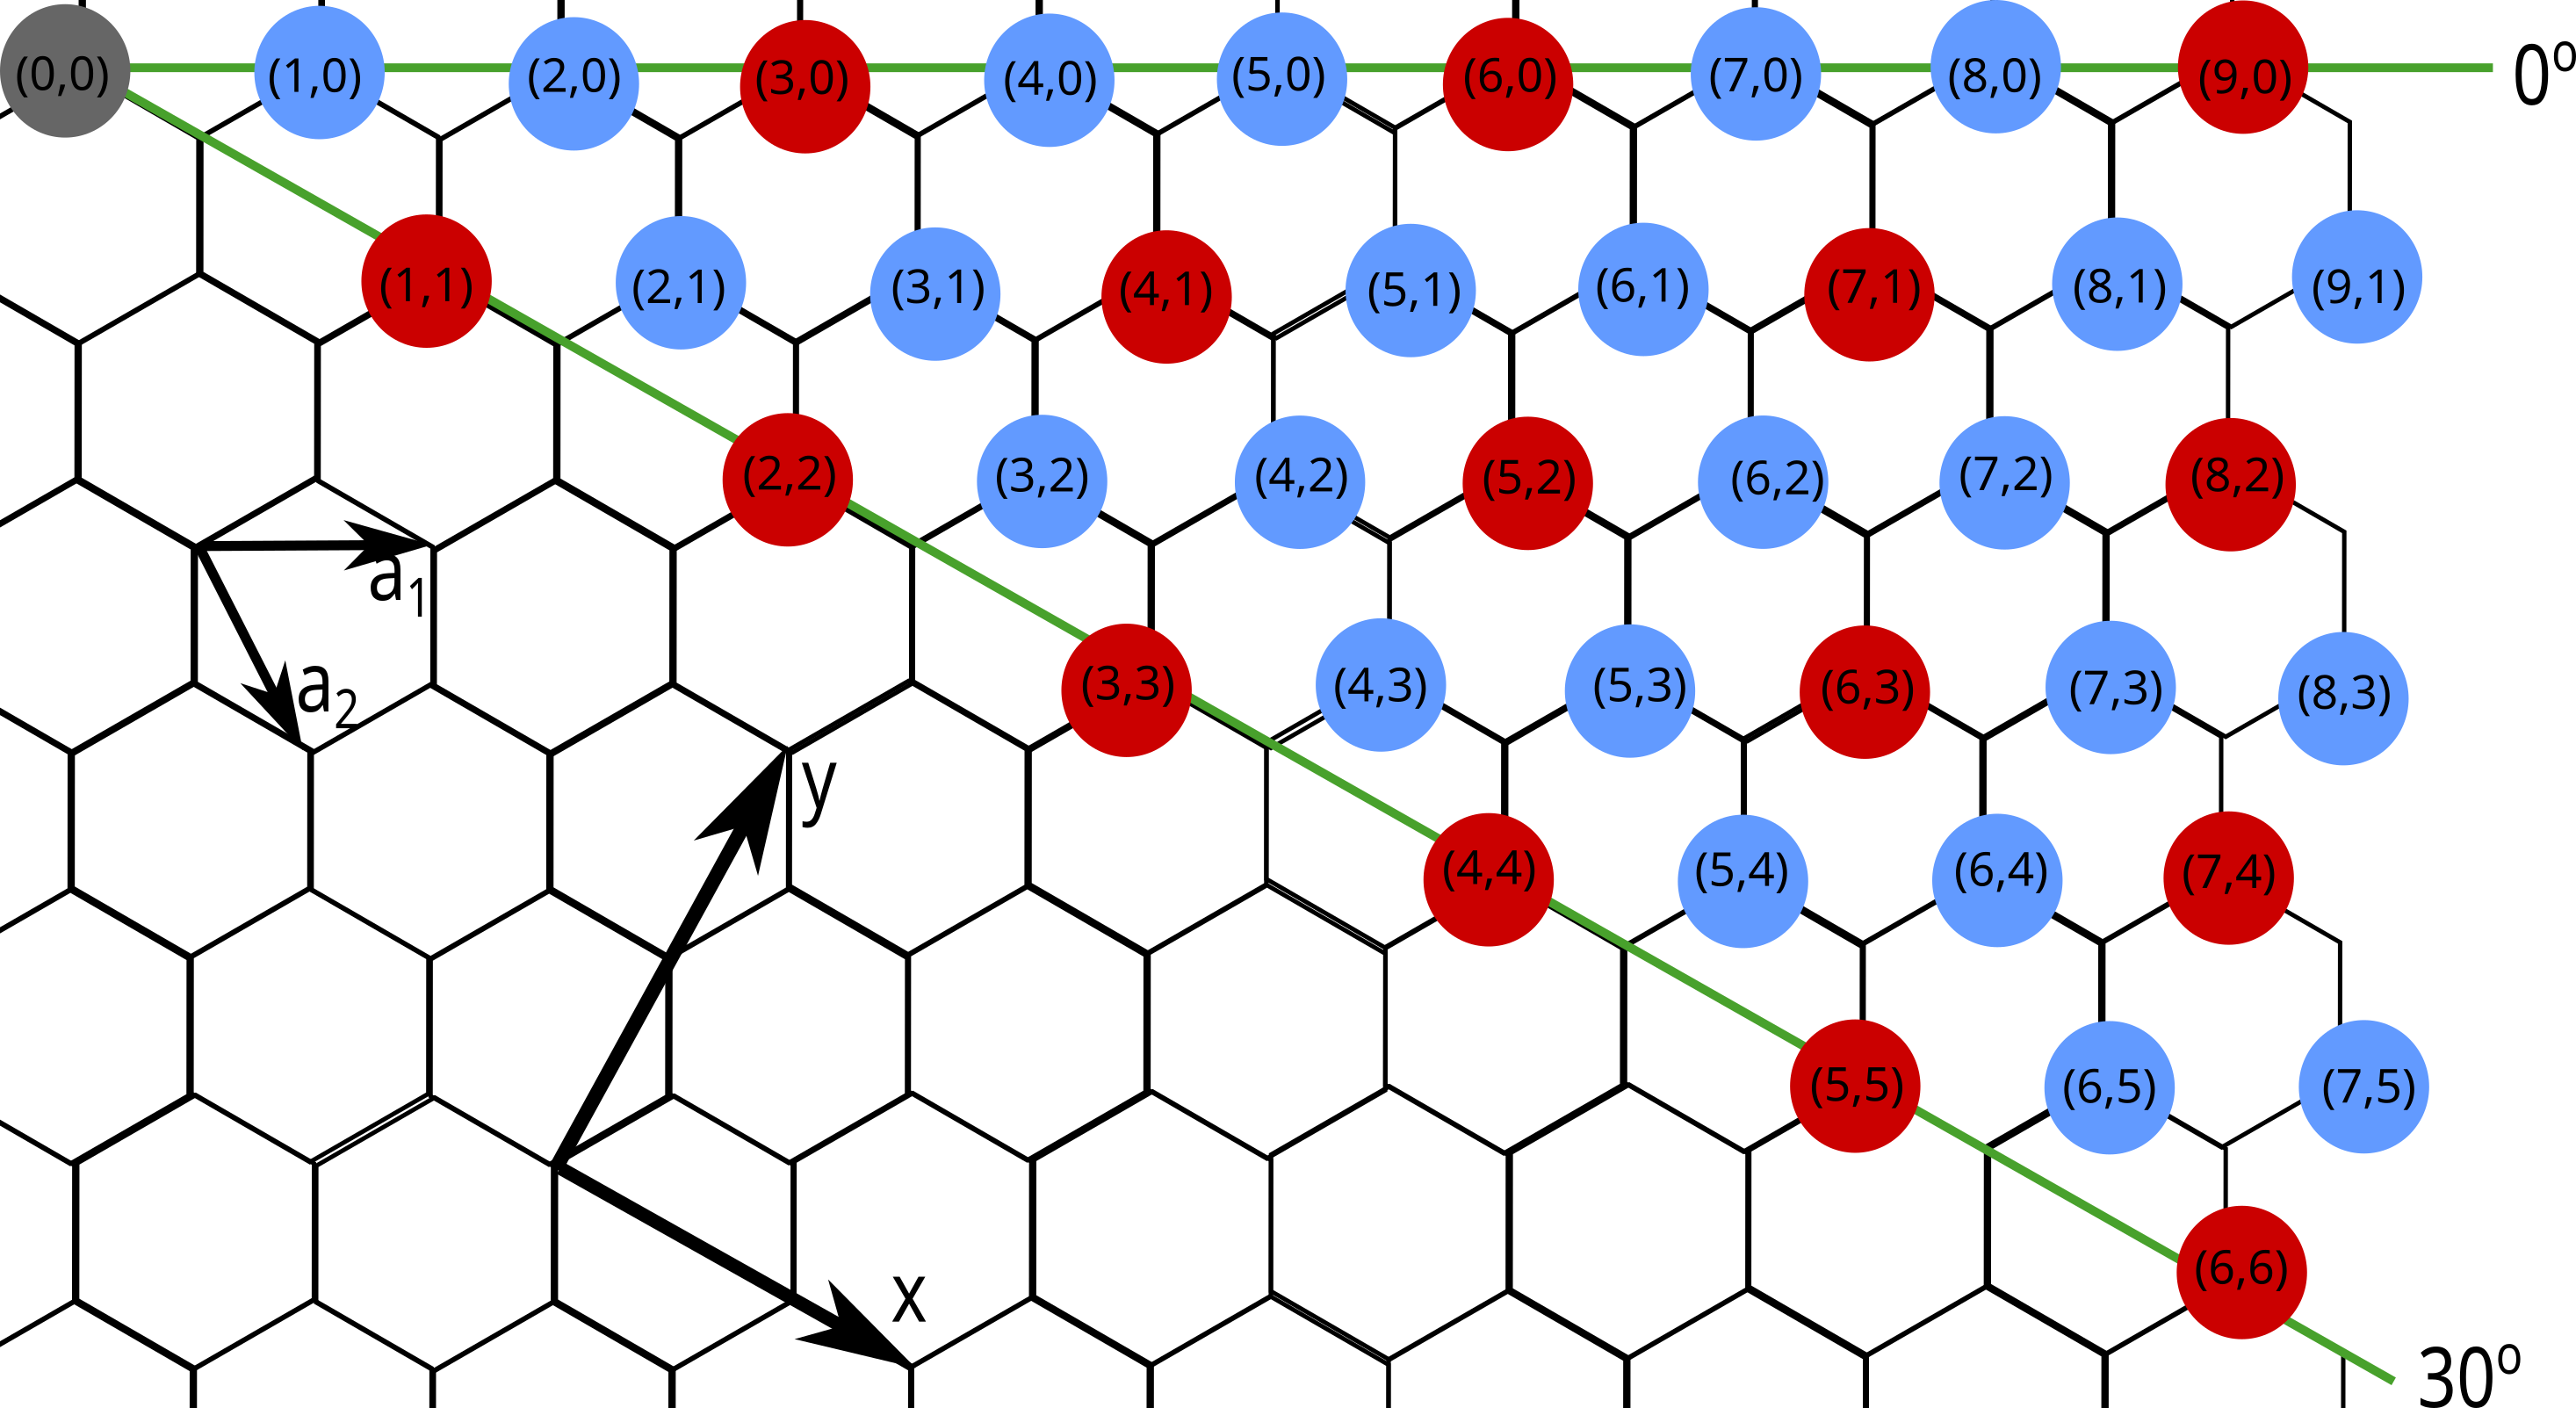
\includegraphics[width=0.5\textwidth]{./Figures/CNTs/chiral.png}
	\caption{REPLACE Chiralities of CNTs with red dots indicating metallic and open dots  \cite{dresselhaus}. }
	\label{fig:chiralities}
\end{figure}

\begin{figure}[h]
	\centering
	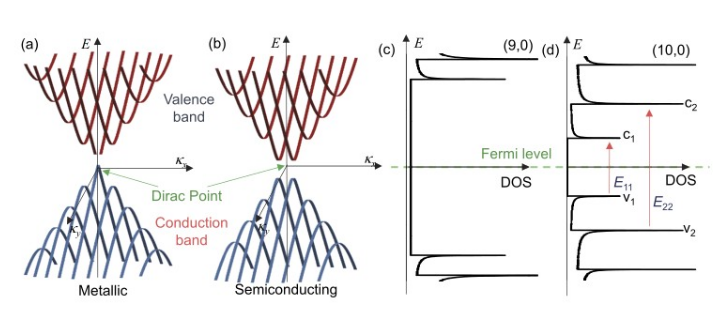
\includegraphics[width=0.5\textwidth]{./Figures/CNTs/DOS.png}
	\caption { REPLACE Bands for (a)(c)Metallic and (b)(d)Semiconducting CNTs and their energy band gaps \cite{yamashita}}
	\label{fig:cnt dos}
\end{figure}
\clearpage
% TODO: Figure 4 is not indicated correctly here
In the same year as the emergence of CNTs as a unique material, H. Kataura measured the optical absorption spectra of CNTs of various diameter CNTs performing photothermal deflection spectroscopy, which measures heat produced during relaxation of the electron hole pair generated by the absorbed light \cite{kataura}; Examples of the optical absorption spectra are shown in Figure 4. While the absorption spectra across various CNT samples were consistent, the peak positions varied. Using the energy dispersion relations for pi-bands of the graphite \cite{kataura}
\begin{equation}
	E_{2D} = \pm\gamma\sqrt{1+4cos(\frac{\sqrt{3}k_x a}{2})cos(\frac{k_y}{2}) + 4cos^2(\frac{k_y}{2}) }
\end{equation}
where  is the overall integration and ,  are the reciprocal lattice vectors, fulfilling the periodic boundary condition for chiral vectors from Eq. (5), the one-dimensional energy band of CNTs could be calculated. Referring to Figure3, the spikes in the DOS correspond to the energy levels of the optical transitions. Plotting the Gap energies from this model against the nanotube diameter in Figure5, referred to commonly as a Kataura plot, shows how the first transition energy of CNTs has a relationship to the diameter by
\begin{equation}
	E_{11} = \frac{2\gamma a_{C-C}}{d}
\end{equation}
and the average band gap energies split along semiconductor and metallic chiral values. In short the absorption peak wavelength of a nanotube sample is determined by the mean tube diameter, and the absorption spectral bandwidth will be determined by the tube diameter distribution of the CNT sample.
\begin{figure}[h]
	\centering
	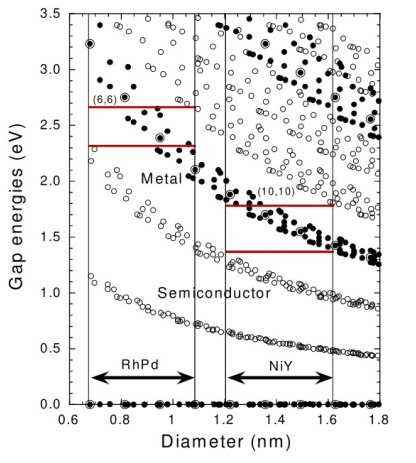
\includegraphics[width=0.5\textwidth]{./Figures/CNTs/kautura.png}
	\caption{Chiralities of CNTs with red dots indicating metallic and open dots  Calculated gap energies between mirror-image spikes in density of states for $\gamma = 2.75$ eV. For (solid circles) metallic  and (open circles) semiconducting, and (double circles) armchair CNTs. \cite{kataura}. }
	\label{fig:kataura}
\end{figure}
\clearpage

\section{Nonlinear Optical Properties of CNTs}
The general relationship between the polarization and electric field of a material is defined \cite{yamashita.tutorial} as
\begin{equation}
	P(t) = \epsilon_0(\chi^{(1)}E(t) + \chi^{(2)}E^2(t) + \chi^{(3)}E^3(t)+...)
\end{equation}

where is the linear susceptibility and are the second and third order susceptibility. Due to the inversion symmetry of the CNT’s structure, the second-order susceptibility is zero. However, a large third-order nonlinearity in CNTs has been measured \cite{martinez} and is theorized to be a product of the one dimensional motion of the delocalized $\pi$-band electrons at a fixed lattice ion configuration \cite{margulis}.  The third-order nonlinearity is responsible for the saturable absorption of a material as well as the nonlinear Kerr effect.
The refractive index as defined (\ref{eq:refractive_index}) is composed of the real part of the third-order susceptibility with $I$ defining the optical intensity and  as the optical angular frequency, and  is the nonlinear refractive index.
\begin{equation}
	n = n_0 + n_2I = n_0 + \frac{3Re[\chi^{(3)}]}{4\epsilon_0cn_0^2}I
	\label{eq:refractive_index}
\end{equation}
The absorption coefficient defined by (\ref{eq:absorption_coefficient}) is composed of the imaginary part of the third-order susceptibility and  ,  and  are the linear absorption coefficient, the non saturable absorption coefficient, and refractive index respectively.
\begin{equation}
	\alpha = \frac{\alpha_0}{1+\frac{I}{I_S}} + \alpha_{int} \sim\alpha_0 + \alpha_{int} + \frac{3\omega Im[\chi^{3}]}{2\epsilon_0c^2n_0^2}I
	\label{eq:absorption_coefficient}
\end{equation}
The saturation intensity, , is the power per unit area it takes in a steady state to reduce the absorption to 1/2 the unbleached (or completely saturated) value and can be written in terms of
\begin{equation}
	I_S = \frac{hf}{\sigma\tau} =\frac{E_S}{\tau}
	\label{eq:saturation_intensity}
\end{equation}

where  $\sigma$ is the absorption cross section and $E_S$ is the saturation fluence, which is the fluence (i.e. energy per unit area) it takes to reduce the initial fluence value to $e^{-1}$ and  $\tau$ is the recovery time of the material.

The saturable absorption, as defined by (\ref{eq:saturation_intensity}), is a phenomenon where high intensity light will reduce the absorption of a material, but at weak intensity, the light will be absorbed and cause attenuation. This property of materials with strong third-order susceptibility like CNTs can be used to filter out weaker optical signals in noisy optical pulses, while simultaneously allowing strong pulses to pass through. Saturable absorption is observed in all materials with optical absorption resulting from electron transition between two energy levels \cite{thomsen}, but it is rare to find materials that have a recovery time that has a fast recovery time compared to the pulse duration, which in ultra-fast laser applications is in the few picosecond to femtosecond range. The ultra-fast response time of CNTs  is only true however for bundles of CNTs with variations in their diameter due to entanglement between semiconducting and metallic via electrons tunneling and coupling from semiconducting CNTs to metallic CNTs \cite{gambetta}.

\section{Fluorescence of CNTs}
The first Van Hove optical transition (E11)
corresponds to the emission frequency and the
second Van Hove optical transition (E22) corresponds
to the excitation frequency. Equations for first and second van Hoven Transitions optical transition wavelengths as a function of diameter in
nanometers and chiral angle are degrees derived in \cite{bachilo}, but  parameters from \cite{weisman}, which were found by fitting
to data of samples of individual SWNT in aqueous sodium dodecyl sulfate (SDS) suspension and are valid for
CNT diameters greater than 0.5nm.
The parameters differ for each CNT “group”, i.e  (n-m) mod 3 = 1 is group 1
(n-m) mod 3 = 2 is group 2
(n-m) mod 3 = 0 are metallic CNTs and do not fluoresce.

Though it is unknown what specific effects contribute to the fitted parameters with the particular samples used, \cite{weisman}found that other
aqueous solutions have comparative spectral shifts of less than 2\% compared to the equations when compared to other published
results. Comparing to an experimental PL map using a different solutio\cite{giordani}, the equation results match quite well (the CNTs present in
the left sample are marked in red on the right plot). We can see the expected variation from different solutions, for example CNT (10,
8) has a slightly higher excitation wavelength and slightly lower emission wavelength in SDS than in the NaDDBS/D2O solutions.

Only fully intact and individually dispersed semiconducting CNTs emit fluorescence
CNTs coatings or placed on a substrate don’t really fluoresce
Interactions between CNTs typically cause quenching effects
Though certain materials/solvents (varies with each CNT) can increase fluorescence
Isolation is one of the largest factors in quantum yield
Only in semiconductor-type CNTs

Desired type of CNTs can be targeted and isolated in a single step using modified aqueous two-phase extraction(ATPS).
Hydration modulating agents are mixed in to tune the arrangement of surfactants on their surface

Depending on the mixture, selected CNTs turn highly hydrophobic or hydrophilic

Spectral shift due to the change in the local dielectric environment surrounding CNTs created by solvents and adsorbed molecules.\cite{turek}

% TODO: check if "1e7" is correct in formula below or should be e^7. It just looks weird to me

\begin{equation}
	(Emission)\lambda_{11} = \Bigg[\frac{1e7(cm^{-1})}{157.5+1066.9d_t} - 771(cm^{-1})\frac{cos(3\theta)^{1.374}}{d_t^{2.272}} \Bigg]^{-1}
\end{equation}
\begin{equation}
	(Excitation)\lambda_{22} = \Bigg[\frac{1e7(cm^{-1})}{145.6+575.7d_t} + 1326(cm^{-1})\frac{cos(3\theta)^{0.828}}{d_t^{1.809}} \Bigg]^{-1}
\end{equation}

\begin{equation}
	(Emission)\lambda_{11} = \Bigg[\frac{1e7(cm^{-1})}{157.5+1066.9d_t} + 347(cm^{-1})\frac{cos(3\theta)^{0.886}}{d_t^{2.129}} \Bigg]^{-1}
\end{equation}
\begin{equation}
	(Excitation)\lambda_{22} = \Bigg[\frac{1e7(cm^{-1})}{145.6+575.7d_t} - 1421(cm^{-1})\frac{cos(3\theta)^{1.110}}{d_t^{2.497}} \Bigg]^{-1}
\end{equation}

\subsection{Group 1 v. Group 2}
Group 1 CNTs have lower Stokes shifts, and small chiral angles (< 2o).
On the other hand, group 2 have higher Stokes shift and span full 0o to 30o chiral angle range, but are grouped along chiral number difference (n - m).

\subsection{Excitation/Emission wavelengths}
% TODO: this section is incomplete. Should also specify what is the "lower plot" by referencing the figure.
Increase in Stokes shifts with diameter along chiral difference (n - m) lines.
Noted in red on lower plot, connected by black lines.
Increase in ex/em wavelengths with diameter
\begin{figure}[h]
	\centering
	\foreach \x in {degrees, diameter}
		{
			\begin{subfigure}[b]{0.49\textwidth}
				\includegraphics[width=\textwidth]{./Figures/CNTs/\x.png}
				\caption{}
			\end{subfigure}
			\hfil
		}
	\caption { Group characteristics of CNTs colored by (a)chiral angle and (b)diameter }
	\label{fig:cnt fluorescence}
\end{figure}
\clearpage
